The user interface (UI), as shown in \Cref{fig:generic_ui}, is where the analysis
is configured and managed. Here, the user is able to provide the necessary
parameters to create the simulation, start the simulation both locally and
remotely, and view the simulation results. The interface contains several
separate areas:

\softwareSwitch{PBE}{
\begin{figure}[!htbp]
  \centering {
    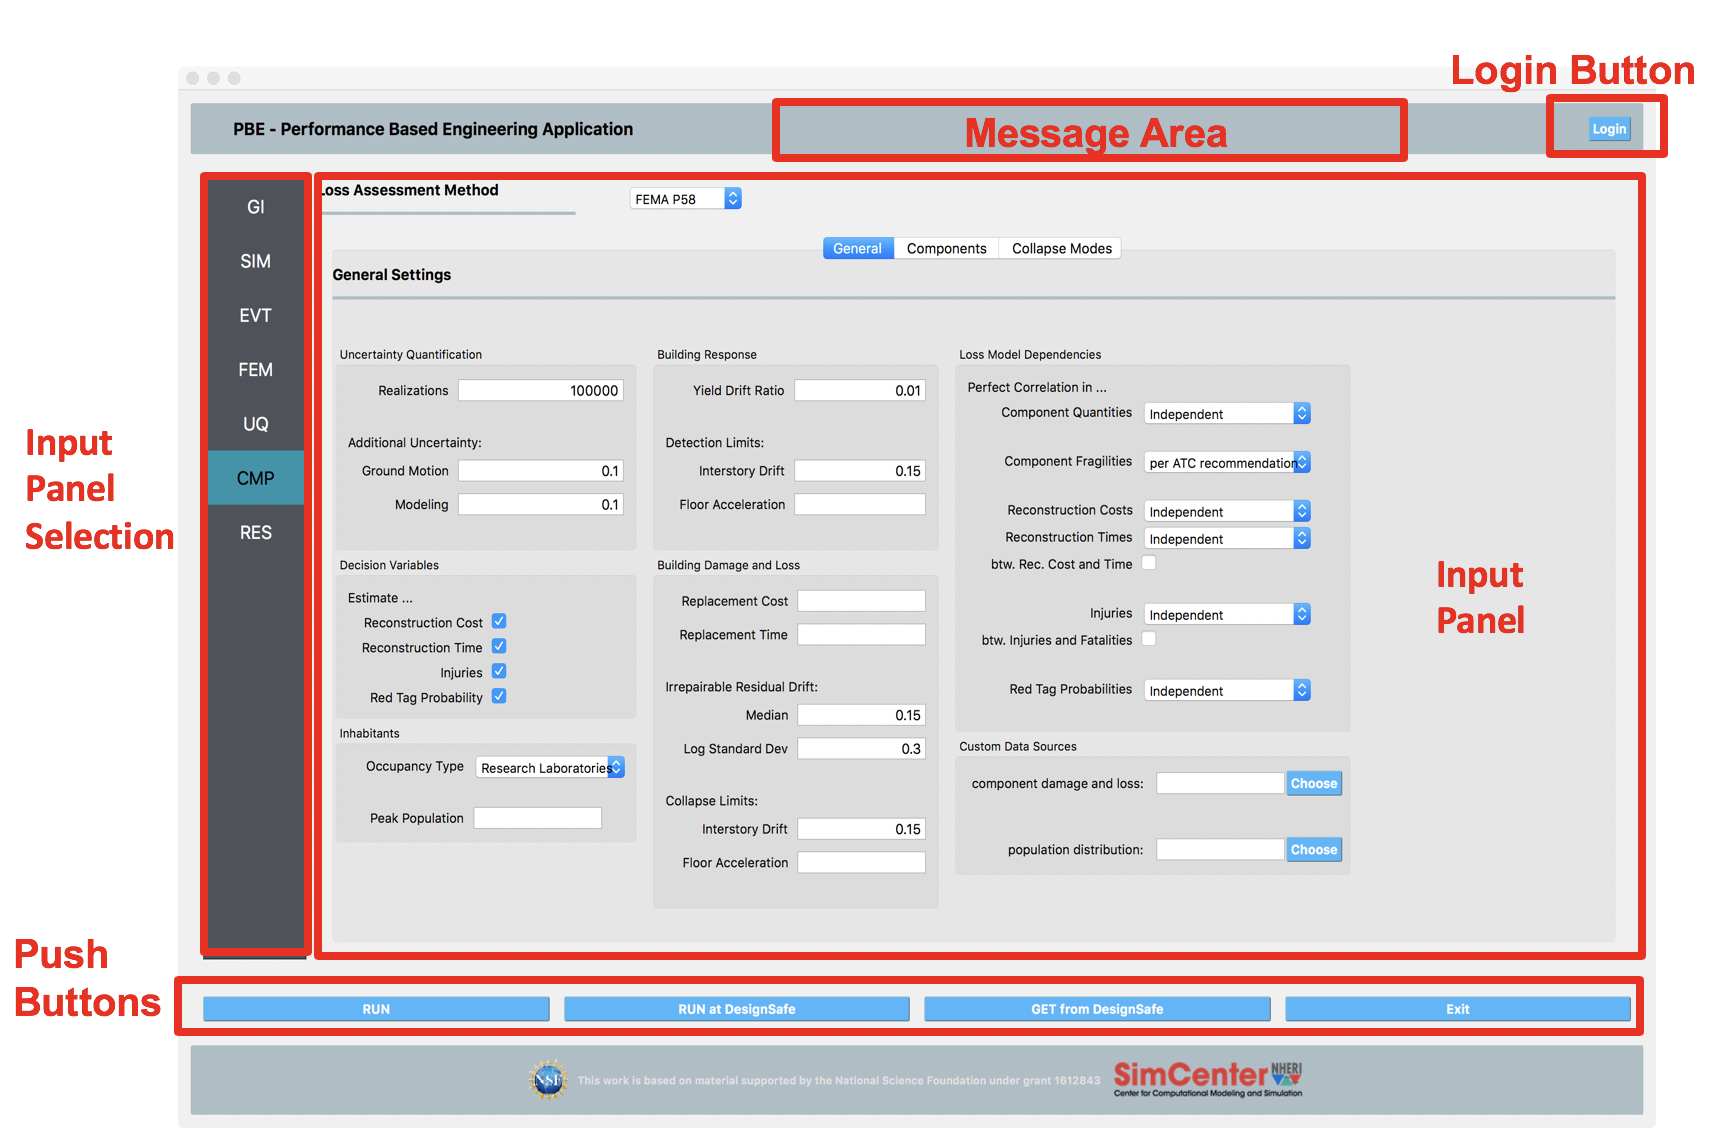
\includegraphics[width=0.95\textwidth]
    {usage/figures/pbePanel.png} }
  \caption{The User Interface (UI)}
  \label{fig:generic_ui}
\end{figure}
}{
\begin{figure}[!htbp]
  \centering {
    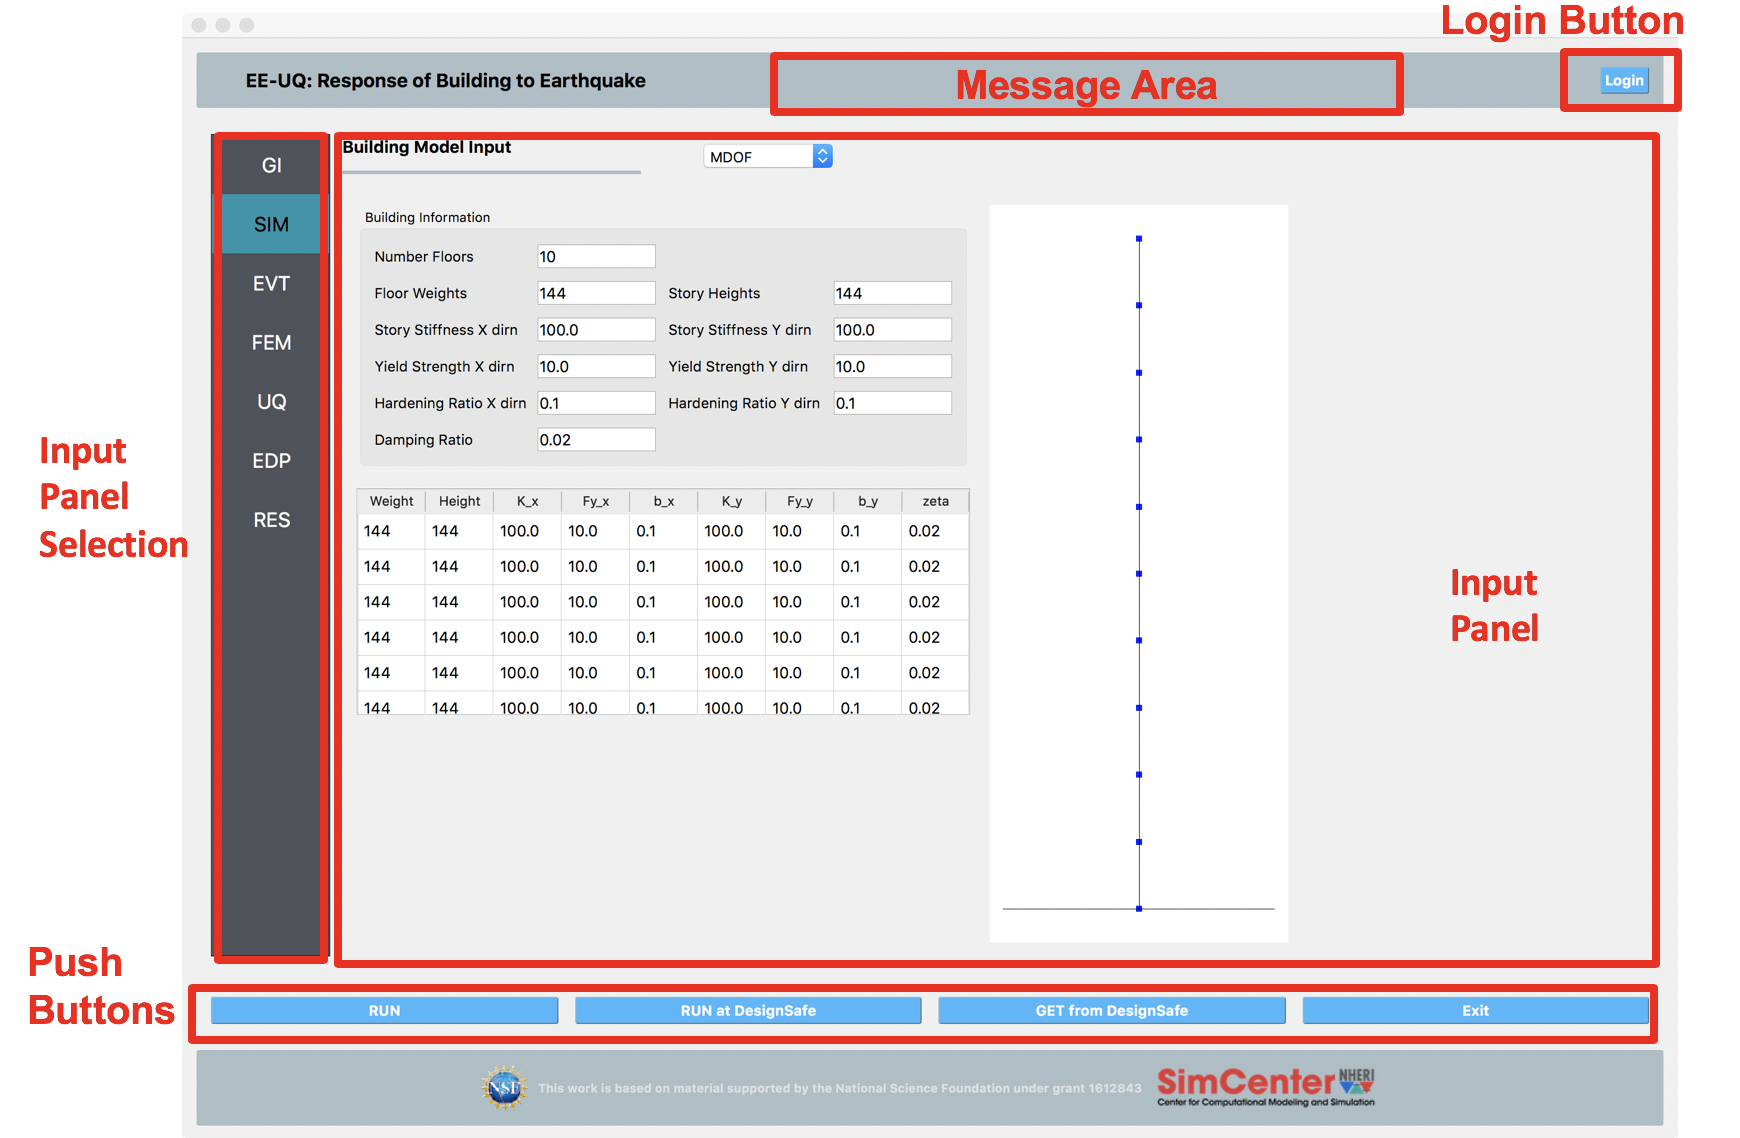
\includegraphics[width=0.95\textwidth]
    {usage/figures/eePanel.png} }
  \caption{The User Interface (UI)}
  \label{fig:generic_ui}
\end{figure}
}

\begin{enumerate}
\item Input Panel Selection: This area on the left side provides the
  user with a selection of items to choose from:
\begin{enumerate}
  \item GI: General Information (\Cref{sec:generalInfo}), for specification of building
    description, location and units.
  \item SIM: Structure Information Model (\Cref{sec:structuralInfo}), for description of the
    building model.
  \item EVT: Event (\Cref{sec:event}), for selecting the input earthquake motions for the building.
  \item FEM: Finite Element Method (\Cref{sec:fem}), for specifying the options for structural response simulation.
  \item UQ: Uncertainty Quantification (\Cref{sec:uq}), for defining the distribution
    of the random paramaters and UQ method analysis options.

\softwareSwitch{PBE}{
 \item DL:  Damage and Loss Model (\Cref{sec:dl}), for specification of the damage and loss model parameters.
}{ 
  \item EDP: Engineering Demand Parameters (\Cref{sec:edp}), for 
  specification of output response quantities.
}

  \item RES: Results output (\Cref{sec:results}), for looking at the results.
\end{enumerate}

Selecting any of these will change the input panel presented.

\item Input Panel: This is the large central area of the UI where the
  user provides input for the application chosen and views the
  results. For example, if the user had selected UQ in the input panel
  selection, it is in this panel that the user would provide details
  on the distributions associated with each random variable or select
  the sampling method to use and provide the options necessary to run
  that method.

\item Push Buttons: This is the area near the bottom of the UI in
  which 4 buttons are presented to the user:

\begin{enumerate}
\item RUN – Run the simulation locally on the user’s desktop machine.
\item RUN at DesignSafe – Process the information, and send to
  DesignSafe. The simulation will be run there on a supercomputer, and results
  will be stored in the user's DesignSafe jobs folder.
\item GET from DesignSafe – Obtain the list of
  jobs for the user from DesignSafe and select a job to download from that list.
\item Exit: Exit the application.
\end{enumerate}

The first 3 of the above buttons and their use are discussed in more detail in \Cref{sec:push_buttons}.

\item Login Button: The Login Button is at the top right of the UI. Before the user can launch any jobs on DesignSafe, they must
  first login to DesignSafe using their DesignSafe login and
  password. Pressing the login button will open up the login window
  for users to enter this information. Users can register for an
  account on
  the \href{https://www.designsafe-ci.org/account/register/}{DesignSafe
  webpage}.

\item Message Area: While the application is running, error and status messages will be displayed here, in the top center of the user interface.

\end{enumerate}